\documentclass[11pt, a4paper]{article}
\usepackage{graphicx}
\usepackage{amsmath}
\usepackage{listings}


\title{Assignment 3: Fitting Data To Models}
\author{Sakthi Harish D T (Roll No.EE19B054)}
\date{March 3, 2021}

\begin{document}

\maketitle {\textbf{\hspace{50 mm}Report}}

\section*{\hspace{30 mm}:Abstract of Assignment:}
The aim of the assignment is to,
\begin{itemize}
    \item Load data from a file and process the extracted data.
    \item Make plots for the data extracted.
    \item Use the Least Square Function to acquire best fit for the function.
    \item Find the relation between the error and noise that is added to the data.
\end{itemize}

\section{Data Generation}
The data required is generated by running the \textbf{"generate\_code.py"} script file. The generated data is stored in \textbf{"fitting.dat"}. The data consists of one column of time entries and 9 columns of data each with a different amount of noise added to it. Each column of data is of the function \textit{f(t)}, given by,
\begin{equation}\label{eq:1}
f(t) = 1.05J_{2}(t) - 0.105t + n(t)
\end{equation}
\section{Data Analysis}
The actual function to be fitted is given by,
\begin{equation}\label{eq:2}
f(t) = 1.05J_{2}(t) - 0.105t
\end{equation}
where \textbf{$J_2(t)$} is the \textit{Bessel function of second order}. 
The python function \texttt{g(t,A,B)} is defined such that it returns the value of \textbf{f(t)} for the given \textit{A,B} at time instant \textit{t}. 
The time is obtained from the column 1 of the data file.\\
\begin{verbatim}
    def g(t, A, B):
        g= A*sp.jn(2,t) + B*t
        return g
\end{verbatim}

Figure 0 for Q4 is given by the below plot.
The plot contains all the nine columns of data with some noise added to it along with the true value of the function.
  \begin{figure}[!tbh]
   	\centering
   	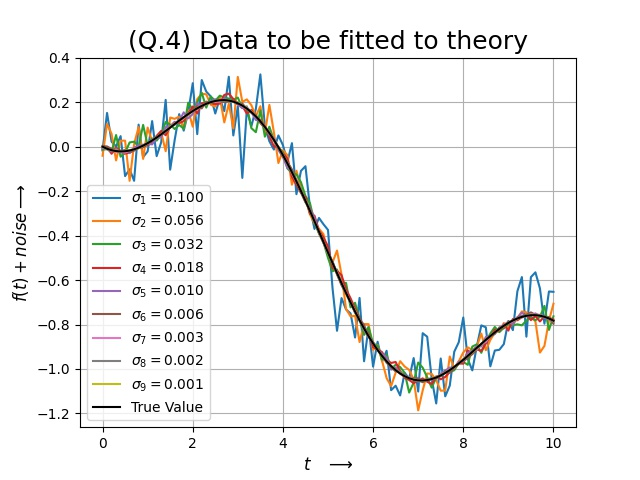
\includegraphics[scale=0.8]{q4.jpeg} 
   	\caption{Noisy Data with True Data}
   	\label{fig:fig1}
   \end{figure} 

As we can see from Figure~\ref{fig:fig1}, the “noisiness” of the data increases with increasing value of $\sigma$. 

Another view of how the noise affects the data can be seen below: 

  \begin{figure}[!tbh]
   	\centering
   	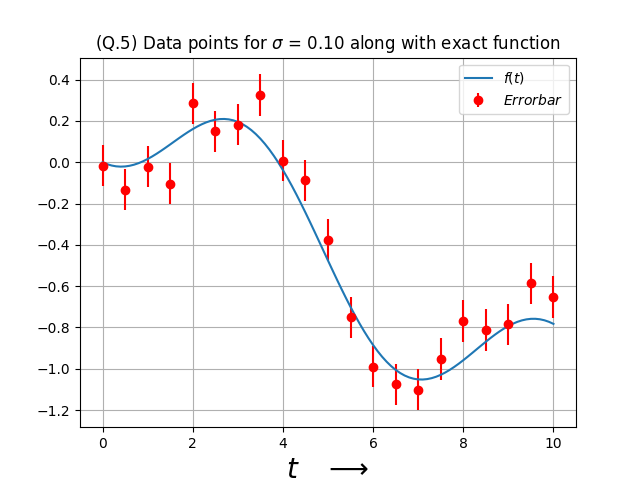
\includegraphics[scale=0.8]{q5.png}  
   	\caption{Noisy Data with Errorbar}
   	\label{fig:fig2}
   \end{figure} 
   
The blue lines (error bar) indicate the deviation of the noisy data from the original data, at that value of t. It is plotted at every 5th point to make the plot readable else the plot would have been clumsy.

\section{Matrix Representation of the equation}
The function which we need to approximate can also be computed by means of a matrix equation. We obtain the function $g(t,A,B)$ as a column vector using the following matrix equation:
\begin{equation}\label{eq:3}
    g(t,A,B) = M.p
\end{equation}
where the matrix
\begin{equation}
M=\left[\begin{matrix}
J_2(t_1)&t_1\\
...&...\\
J_2(t_m)&t_m
\end{matrix}\right]\text{, }
p=\left[\begin{matrix}
A\\B
\end{matrix}\right]
\end{equation}

While performing the computation of the function we generate the matrix M and compute $M.p$ and get the function output.

\section{Best fit approximation to the noisy data}

From the data given to us we see that, we must approximate the noisy data to a function of the form:

\begin{equation}\label{eq:4}
    g(t, A, B) = AJ_2(t)+Bt
\end{equation}

where we must find the values of the constants A and B by using the least square estimation. For this purpose we take the value of A = 0,0.1,0.2,...,2 and B = -0.2,-0.19,...,0 and iterate through each of the above values of A and B, and finally get the mean squared error between the given noisy data and the approximated function by taking the each pair of above values of A and B. 
\newline

The error is computed by means of the following equation:
\begin{equation}\label{eq:5}
    \epsilon_{ij} = \frac{1}{101}\sum_{k=0}^{101}(f(t_k) - g(t_k, A_i, B_j))^2
\end{equation}

where $\epsilon_{ij}$ is the error for $(A_i,B_j)$.

After computing the mean squared error we plot a contour plot for the same with the values of A and B on the x-axis and y-axis respectively. The plot is as shown below:

\begin{figure}[!tbh]
   	\centering
   	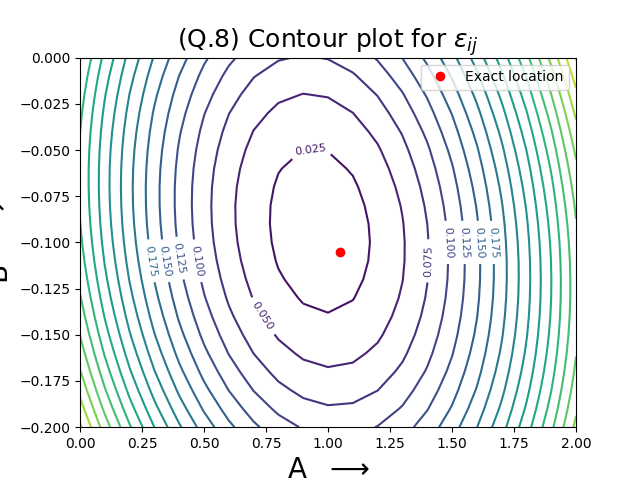
\includegraphics[scale=0.8]{q8.png}  
   	\caption{Contour Plot of $\epsilon_{ij}$}
   	\label{fig:fig3}
   \end{figure} 
   
  We can find that the plot has a minimum.  
\section{The Least Square Fitting Model}

We are required to find the best measure estimate for the constants A and B in the equation \eqref{eq:3} for the noisy data. We do this by applying the method of least square estimation. This is implemented in python by using the \texttt{lstsq()} function from the \texttt{scipy} package. We pass the matrix M and the noisy data as the input to the \texttt{lstsq()} function and we get the best fit values of A and B. We perform this for all the 9 random noise added data.
\newline

We then compute the mean squared error in the coefficients A and B to their actual value of \texttt{A0 = 1.05} and \texttt{B0 = -0.105} and plot the same  against the standard deviation of the random noise. The plot is shown below:

\begin{figure}[!tbh]
   	\centering
   	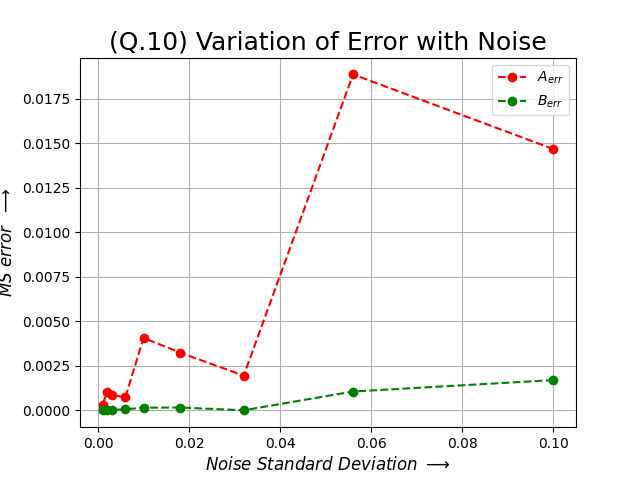
\includegraphics[scale=0.8]{q10.png} 
   	\caption{Mean squared error vs Noise Standard deviation}
   	\label{fig:fig4}
   \end{figure} 

\newline
\newline
We aren't able to seek in much information to get a relation between $\sigma and$ $\epsilon$ from the above plot. If we plot the same in \texttt{log-log} scale along with their error bar, the plot looks like as shown in Figure 5.
\newline
\newline
\newline
\newline
\newline

\begin{figure}[!tbh]
   	\centering
   	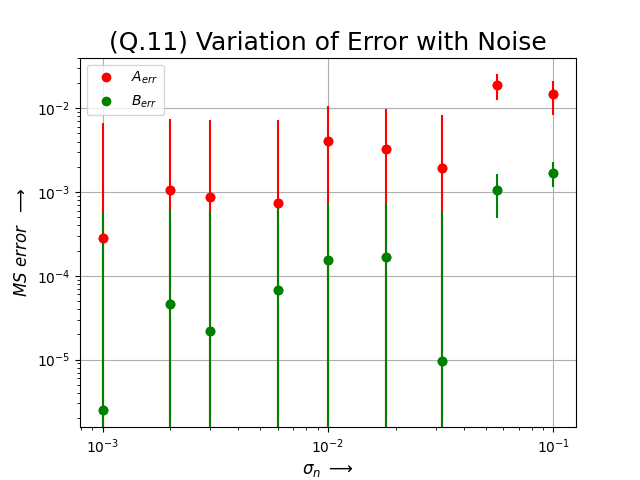
\includegraphics[scale=0.8]{q11.png} 
   	\caption{Mean squared error vs Noise Standard deviation log-log plot}
   	\label{fig:fig5}
   \end{figure} 
 \newline
 From the below plot we can infer that there is a linear relation between $\sigma_n$ and $\epsilon$, which is the required result to be produced.

\section{Conclusion}
We have used the given noisy data and computed the best possible for the underlying model parameters by minimizing the mean squared error. By plotting the mean squared error between the estimated model parameters A and B and the true value function's parameters A0 and B0, we see that this error is varying linearly with the standard deviation of the noise added to true value.

Also, the least square model is a very good tool for fitting models.
\end{document}

    
    



\end{document}

